% ============================================================
%  GamefyDB — PFE Report  |  Chapters 4, 5 & 6 + Conclusion
%  Append this content inside the main document, before \end{document}
% ============================================================

% ============================================================
%  CHAPTER 4
% ============================================================
\chapter{Sprint 2: Star Schema and Data Export}

\section{Introduction}

Sprint~2 builds on the clean DataFrames produced in Sprint~1. Its scope covers user
stories US-05 through US-07: constructing the four dimension tables and the two fact
tables that make up the GamefyDB star schema, then writing everything to disk in the
format Power~BI expects. By the end of the sprint, the pipeline is end-to-end: raw
Excel files go in, a ready-to-load star schema comes out.

\section{Sprint 2 Backlog}

Table~\ref{tab:sprint2_backlog} lists the tasks committed to this sprint.

\begin{longtable}{>{\bfseries}p{1.3cm} p{4.2cm} p{7cm}}
  \caption{Sprint 2 Backlog.\label{tab:sprint2_backlog}} \\
  \toprule
  \textbf{ID} & \textbf{User Story} & \textbf{Tasks} \\
  \midrule
  \endfirsthead
  \toprule
  \textbf{ID} & \textbf{User Story} & \textbf{Tasks} \\
  \midrule
  \endhead
  \bottomrule
  \endfoot

  US-05 & As an analyst, I want four normalised dimension tables with surrogate keys.
        & Build \textit{dim\_cashier}, \textit{dim\_terminal}, \textit{dim\_item},
          and \textit{dim\_member} from the cleaned DataFrames; assign sequential
          integer primary keys. \\[4pt]

  US-06 & As an analyst, I want two fact tables with foreign-key references to the
          dimensions.
        & Build \textit{fact\_transaction} from the cash data and
          \textit{fact\_session} from the sessions data; resolve FK references to
          all four dimension tables. \\[4pt]

  US-07 & As an analyst, I want to export the full star schema as CSV files ready
          for Power~BI.
        & Implement the export step in \texttt{run.py}; write each table to
          \texttt{output/powerbi\_star/} with UTF-8-BOM encoding so Power~BI
          reads French characters correctly. \\
\end{longtable}

\section{Design Refinement}

During Sprint~0, the product backlog described eight output tables — four dimensions
and four fact tables. After inspecting the actual source data more carefully during
Sprint~1, the design was refined:

\begin{itemize}
  \item \textbf{Stock movements} were absorbed into \textit{dim\_item}. All stock
        records in the source file are outgoing sales — there are no restock entries.
        Because there is only one direction of movement, a dedicated fact table adds
        no analytical value; instead, quantity sold and total revenue are aggregated
        directly into the item dimension.

  \item \textbf{Member statistics} were kept as \textit{dim\_member}. The members
        file contains one summary row per member — cumulative totals, not individual
        events — so it naturally fits a dimension rather than a fact table.
\end{itemize}

The final schema therefore has six tables: four dimensions and two facts. This
simplification makes the Power~BI data model easier to navigate without losing any
of the required KPIs.

\section{Implementation of the Transformer Stage}

\subsection{Building the Dimension Tables}

\subsubsection{dim\_cashier}

The cashier dimension is built by collecting all distinct cashier names across the
three transactional domains — cash, sessions, and stock — sorting them alphabetically,
and assigning a sequential surrogate key starting at~1. The five cashier accounts
in the source data (\textit{guds}, \textit{monta}, \textit{taktek},
\textit{yassine}, \textit{youssef}) all appear in the result.

\subsubsection{dim\_terminal}

The terminal dimension is derived exclusively from the sessions file, since that is
the only source that records terminal names reliably. Each unique \texttt{(terminal,
terminal\_type)} pair becomes one row. The \texttt{terminal\_type} column is computed
during cleaning: terminals whose names contain \texttt{PS5} become \textit{PlayStation},
those containing \texttt{VIP} become \textit{VIP PC}, and all others become
\textit{Standard PC}. The final dimension contains 16 terminals.

\subsubsection{dim\_item}

The item dimension aggregates the stock table by item name, retaining the first
observed category, the median unit price, total quantity sold, and total revenue.
Median is used instead of mean for the unit price so that occasional data-entry errors
do not distort the representative price. The dimension contains 17 distinct items.

\subsubsection{dim\_member}

The member dimension is a direct copy of the cleaned members DataFrame with no
further aggregation. It contains 66 unique members, each described by their username,
first name, last name, cumulative session duration in minutes, and cumulative spend
in TND across usage, orders, USB data, and total.

\subsection{Building the Fact Tables}

\subsubsection{fact\_transaction}

The transaction fact table is built from the cash DataFrame. Each row represents one
cash register event — an income or expense entry recorded by a cashier. The foreign
key resolution works as follows:

\begin{itemize}[noitemsep]
  \item \textbf{cashier\_id} — looked up from the cashier name map built from
        \textit{dim\_cashier}.
  \item \textbf{terminal\_id} — assigned only for \textit{Computer Incomes} and
        \textit{Playstation Incomes} categories, since those are the only transaction
        types tied to a terminal. Rows in other categories carry a null terminal
        reference.
  \item \textbf{item\_id} — assigned only for \textit{Order Incomes} rows, by
        matching the transaction amount to the nearest item unit price in
        \textit{dim\_item}.
  \item \textbf{member\_id} — assigned only for \textit{Member Transactions} rows.
\end{itemize}

The table contains 3\,971 rows after cleaning.

\subsubsection{fact\_session}

The session fact table is built from the sessions DataFrame. Each row is one gaming
session opened at a terminal. The foreign key resolution is more straightforward here:
\texttt{cashier\_id} and \texttt{terminal\_id} are looked up directly by name, since
both columns are already clean strings after the cleaning stage. A \texttt{member\_id}
is assigned to rows whose \texttt{session\_type} is \textit{Member}.

The table retains all financial columns from the sessions source — \texttt{order\_transfer},
\texttt{usb\_data}, \texttt{usage}, \texttt{discount}, and \texttt{total} (all in TND)
— alongside \texttt{duration\_min} and \texttt{session\_type}.

The table contains 6\,285 rows after cleaning.

\subsection{The Export Step}

The output stage is handled by \texttt{run.py}. After \texttt{run\_pipeline()} returns
the schema dictionary, each table is written as a CSV file to
\texttt{output/powerbi\_star/} using UTF-8-BOM encoding (\texttt{utf-8-sig}). This
encoding ensures that Power~BI and Excel both correctly display special characters —
particularly the French names and Arabic-influenced transliterations that appear in
member usernames.

Table~\ref{tab:output_tables} summarises the six output tables and their row counts
for the current dataset.

\begin{table}[H]
  \centering
  \caption{Output tables and row counts.\label{tab:output_tables}}
  \begin{tabular}{llr}
    \toprule
    \textbf{Type} & \textbf{Table} & \textbf{Rows} \\
    \midrule
    Dimension & \texttt{dim\_cashier}    &   5 \\
    Dimension & \texttt{dim\_member}     &  66 \\
    Dimension & \texttt{dim\_item}       &  17 \\
    Dimension & \texttt{dim\_terminal}   &  16 \\
    Fact      & \texttt{fact\_transaction} & 3\,971 \\
    Fact      & \texttt{fact\_session}   & 6\,285 \\
    \bottomrule
  \end{tabular}
\end{table}

\section{Sprint 2 Review}

\subsection{Deliverables}

\begin{itemize}
  \item \textbf{Star schema} — six CSV files in \texttt{output/powerbi\_star/},
        each correctly typed and encoded.
  \item \textbf{Referential integrity} — every foreign key in \textit{fact\_transaction}
        and \textit{fact\_session} references a valid primary key in the corresponding
        dimension, with null values used only where no meaningful reference exists
        (e.g.\ transactions unrelated to a terminal).
  \item \textbf{End-to-end pipeline} — a single \texttt{python run.py} command
        reads the four source files and produces all six output tables with no
        manual steps.
\end{itemize}

\subsection{Validation}

The output tables were loaded into Power~BI and the data model relationships were
defined. Validation checks included:

\begin{itemize}[noitemsep]
  \item No orphaned foreign keys in either fact table.
  \item Total revenue computed from \textit{fact\_transaction} matches the sum
        visible in the raw cash file.
  \item Terminal names in \textit{fact\_session} join correctly to
        \textit{dim\_terminal} for all 16 terminals.
  \item Member IDs in \textit{dim\_member} cover all 66 distinct members that
        appear in the source.
\end{itemize}

\section{Conclusion}

Sprint~2 produced a complete, validated star schema that Power~BI can consume
directly. The design refinement from eight to six tables simplified the data model
without losing any analytical capability. Chapter~5 describes how this schema is used
to build the interactive dashboards.

% ============================================================
%  CHAPTER 5
% ============================================================
\chapter{Sprint 3: Power~BI Dashboards}

\section{Introduction}

With a clean star schema available, Sprint~3 focuses on turning the data into visual
insights. The deliverable is an interactive Power~BI report (\texttt{gamefyyy.pbix})
with four thematic pages, each targeting a different operational question. The
measures are written in DAX (Data Analysis Expressions), Power~BI's formula language
for calculated columns and aggregations.

\section{Sprint 3 Backlog}

Table~\ref{tab:sprint3_backlog} lists the tasks committed to this sprint.

\begin{longtable}{>{\bfseries}p{1.3cm} p{4.2cm} p{7cm}}
  \caption{Sprint 3 Backlog.\label{tab:sprint3_backlog}} \\
  \toprule
  \textbf{ID} & \textbf{User Story} & \textbf{Tasks} \\
  \midrule
  \endfirsthead
  \toprule
  \textbf{ID} & \textbf{User Story} & \textbf{Tasks} \\
  \midrule
  \endhead
  \bottomrule
  \endfoot

  US-08 & As an analyst, I want to visualise revenue, sessions, stock, and
          member KPIs in Power~BI.
        & Import all six CSV tables; define the data model relationships; create
          \textit{dim\_date}; write all DAX measures; build four dashboard pages
          with slicers. \\
\end{longtable}

\section{Data Model Setup}

\subsection{Relationships}

After importing the six CSV tables, the following relationships were defined in
Power~BI's Model view:

\begin{itemize}[noitemsep]
  \item \texttt{dim\_cashier[cashier\_id]} $\rightarrow$
        \texttt{fact\_transaction[cashier\_id]} (one-to-many)
  \item \texttt{dim\_cashier[cashier\_id]} $\rightarrow$
        \texttt{fact\_session[cashier\_id]} (one-to-many)
  \item \texttt{dim\_terminal[terminal\_id]} $\rightarrow$
        \texttt{fact\_transaction[terminal\_id]} (one-to-many)
  \item \texttt{dim\_terminal[terminal\_id]} $\rightarrow$
        \texttt{fact\_session[terminal\_id]} (one-to-many)
  \item \texttt{dim\_item[item\_id]} $\rightarrow$
        \texttt{fact\_transaction[item\_id]} (one-to-many)
  \item \texttt{dim\_member[member\_id]} $\rightarrow$
        \texttt{fact\_transaction[member\_id]} (one-to-many)
  \item \texttt{dim\_member[member\_id]} $\rightarrow$
        \texttt{fact\_session[member\_id]} (one-to-many)
\end{itemize}

\subsection{Date Dimension}

Power~BI's time intelligence functions (month-over-month comparisons, date-based
slicers) require a dedicated calendar table. A \textit{dim\_date} table was created
as a calculated table covering the full date range of \textit{fact\_transaction},
enriched with columns for year, month number, month name, day, weekday name, and
week number. This table was marked as a date table and linked to the date column of
\textit{fact\_transaction}.

Two calculated columns were added directly to \textit{fact\_transaction}:
\textbf{Transaction Hour} (the hour part of the datetime, used in hourly bar charts)
and \textbf{Transaction Date} (the date part only, used in today-filtered KPIs).

\section{KPI Measures}

The following key measures were defined. They are used across the four dashboard
pages as context allows.

\begin{table}[H]
  \centering
  \caption{Core DAX measures defined in the report.}
  \begin{tabular}{ll}
    \toprule
    \textbf{Measure} & \textbf{Description} \\
    \midrule
    Total Revenue          & Sum of income transactions (TND) \\
    Total Expenses         & Sum of expense transactions (TND) \\
    Net Income             & Total Revenue minus Total Expenses \\
    Revenue MoM\%          & Month-over-month revenue growth rate \\
    Transaction Count      & Count of income transactions \\
    Avg Ticket             & Average revenue per income transaction \\
    Avg Daily Revenue      & Revenue divided by number of distinct active days \\
    \midrule
    Session Count          & Total rows in \textit{fact\_session} \\
    Session Revenue        & Sum of session totals (TND) \\
    Avg Session Duration   & Average session length in minutes \\
    Avg Session Revenue    & Session Revenue divided by Session Count \\
    Discount Total         & Total discount amount granted on sessions \\
    Free Time Sessions\%   & Fraction of sessions flagged as free-time \\
    \midrule
    Item Units Sold        & Total units of stock sold (Out movements) \\
    Item Sales Revenue     & Total revenue from stock sales (TND) \\
    Current Stock          & Net stock level per item (In minus Out) \\
    \midrule
    Revenue Today          & Total Revenue filtered to today's date \\
    Net Income Today       & Net income for today \\
    Transactions Today     & Transaction count for today \\
    \bottomrule
  \end{tabular}
\end{table}

\section{Dashboard Pages}

The report is structured into four pages, each answering a specific operational
question.

\subsection{Page 1 — Revenue Overview}

This page gives a high-level picture of the center's financial performance.

\begin{itemize}
  \item \textbf{KPI cards}: Total Revenue, Total Expenses, Net Income, and
        Revenue MoM\% give a snapshot of the period selected by the slicers.
  \item \textbf{Revenue over time}: A line chart with the date on the horizontal
        axis shows revenue trends, making seasonal patterns and peaks visible
        at a glance.
  \item \textbf{Revenue by hour of day}: A bar chart using the Transaction Hour
        calculated column shows at which hours of the day the center collects the
        most income. This helps identify the busiest operating windows.
  \item \textbf{Revenue by payment method}: A donut chart breaks down income by
        cash versus credit card, giving a sense of how customers prefer to pay.
  \item \textbf{Slicers}: Month name and year slicers allow filtering the entire
        page to a specific period.
\end{itemize}

\subsection{Page 2 — Rankings}

This page answers the question: \textit{who and what is generating the most value?}

\begin{itemize}
  \item \textbf{Cashier performance}: A horizontal bar chart ranks cashiers by
        Total Revenue so the owner can see at a glance which shifts are most
        productive.
  \item \textbf{Item sales}: A bar chart of Item Sales Revenue by item name shows
        which snack-bar products drive the most income and which are barely moving.
  \item \textbf{Terminal performance}: A clustered bar chart compares session revenue
        across terminal types (Standard~PC, PlayStation, VIP~PC) and a detailed
        table lists every terminal with its session count and total revenue.
  \item \textbf{Session metrics}: KPI cards for Avg Session Duration, Discount Total,
        and Free Time Sessions\% round out the terminal analysis.
\end{itemize}

\subsection{Page 3 — Live Ops}

This page is designed for the start-of-shift review: what happened today?

\begin{itemize}
  \item \textbf{Today's KPIs}: Cards for Revenue Today, Expenses Today, Net Income
        Today, and Transactions Today update automatically to reflect the current
        calendar date without any slicer interaction.
  \item \textbf{Stock movements today}: Cards for Stock In Today and Stock Out
        Today show how much stock moved during the day.
  \item \textbf{Current stock levels}: A table listing each item alongside its
        Current Stock measure (net In minus Out across all time) lets the cashier
        on duty see at a glance which items are running low. Conditional formatting
        highlights negative or near-zero values in red.
  \item \textbf{Sessions by terminal type}: A bar chart gives a quick view of how
        busy each terminal type is today.
\end{itemize}

\subsection{Page 4 — Shift Report}

This page provides a per-cashier, per-date breakdown intended for end-of-shift
reconciliation.

\begin{itemize}
  \item \textbf{Slicers}: A single-select cashier slicer and a date-range slicer
        filter all visuals on the page to a specific cashier and date. All the
        measures defined earlier respond to these slicers automatically.
  \item \textbf{Financial summary}: Cards for Total Revenue, Session Revenue, Item
        Sales Revenue, Shift Net, and Total Expenses give a complete picture of what
        the selected cashier collected.
  \item \textbf{Activity summary}: Cards for Transaction Count, Session Count, Item
        Units Sold, and Discount Total complete the operational view.
  \item \textbf{Breakdown charts}: A bar chart of items sold and a bar chart of
        session revenue by terminal type help the owner understand what drove the
        cashier's numbers for the selected shift.
\end{itemize}

\section{Sprint 3 Review}

\subsection{Deliverables}

\begin{itemize}
  \item \textbf{\texttt{gamefyyy.pbix}} — the fully functional Power~BI report with
        all four pages, all DAX measures, and the complete data model.
  \item \textbf{\texttt{SalesDashboard.pbit}} — a Power~BI template file that can
        be reused to connect the same report to a refreshed dataset.
  \item \textbf{\texttt{docs/dax\_measures.dax}} — the full DAX measure definitions,
        saved separately for documentation and version control.
\end{itemize}

\subsection{Validation}

Each dashboard page was reviewed with the Product Owner. The following checks were
performed:

\begin{itemize}[noitemsep]
  \item Revenue figures on Page~1 were cross-checked against the raw cash file
        totals for a selected month.
  \item Cashier rankings on Page~2 were verified by comparing with manually
        summed figures from the source spreadsheet.
  \item Today's KPIs on Page~3 were confirmed to update correctly when the
        system date was changed in testing.
  \item The Shift Report on Page~4 was tested for three different cashiers; the
        totals matched the per-cashier sums computed externally.
\end{itemize}

\section{Conclusion}

Sprint~3 delivered a four-page interactive Power~BI report that covers revenue,
rankings, live operations, and shift reporting. The Product Owner validated all
pages. With the core BI deliverable complete, the project turned to a fourth sprint
to add forward-looking capabilities through machine-learning forecasting. Chapter~6
covers that work.

% ============================================================
%  CHAPTER 6
% ============================================================
\chapter{Sprint 4: Machine Learning and Analytics}

\section{Introduction}

The first three sprints gave the gaming center something it did not have before: clean,
structured data and a live dashboard to explore it. Sprint~4 takes this a step further
by adding a layer of intelligence to the pipeline. Instead of only showing what
happened, the system can now answer three forward-looking questions: what is likely to
happen next, which customers are the most valuable, and which past days were
statistically unusual.

Three complementary techniques make up this sprint:

\begin{itemize}
  \item \textbf{Time-series forecasting} --- Prophet and SARIMA models predict revenue,
        member activity, and session volume for the next four weeks and three months,
        with confidence intervals that show the plausible range around each estimate.
  \item \textbf{Member segmentation} --- K-means clustering groups the 66 members into
        four behavioural profiles, from Heavy Users to Light Users, based on their
        actual spending and visit patterns.
  \item \textbf{Anomaly detection} --- a statistical Z-score method flags days where a
        metric was unusually high or low relative to the normal pattern for that specific
        day of the week.
\end{itemize}

All three modules feed into the same pipeline. One command reads the source files and
writes eight analytics CSVs ready to load into Power~BI alongside the star schema.

\begin{figure}[H]
  \centering
  % *TODO* Add ML workflow diagram: Star Schema (fact_transaction, dim_member) feeds into forecaster.py / segmenter.py / anomaly_detector.py, each producing CSV outputs, all flowing into Power BI. Draw.io or diagrams.net recommended.
  
\includegraphics[width=0.90\textwidth]{ml_workflow.png}
  \caption{Overview of the Sprint~4 analytics pipeline.\label{fig:ml_workflow}}
\end{figure}

\section{Sprint 4 Backlog}

Table~\ref{tab:sprint4_backlog} lists the tasks committed to this sprint.

\begin{longtable}{>{\bfseries}p{1.3cm} p{4.0cm} p{7.2cm}}
  \caption{Sprint 4 Backlog.\label{tab:sprint4_backlog}} \\
  \toprule
  \textbf{ID} & \textbf{User Story} & \textbf{Tasks} \\
  \midrule
  \endfirsthead
  \toprule
  \textbf{ID} & \textbf{User Story} & \textbf{Tasks} \\
  \midrule
  \endhead
  \bottomrule
  \endfoot

  US-09 & As an owner, I want to see expected revenue for the next 4 weeks and
          3 months so I can plan ahead.
        & Implement \texttt{forecast\_revenue()} using Prophet on daily income
          aggregates; output weekly and monthly projections with confidence
          intervals. \\[4pt]

  US-10 & As an owner, I want to forecast member activity so I know whether
          the loyalty base is growing.
        & Implement \texttt{forecast\_members()} using Prophet on weekly member
          transaction counts; ensure output is a non-negative integer. \\[4pt]

  US-11 & As an owner, I want to know the busiest hours and days so I can
          staff appropriately.
        & Implement \texttt{forecast\_peak\_hours()} computing average transaction
          counts by hour of day and by day of week; export as two separate CSV
          files. \\[4pt]

  US-12 & As an owner, I want to forecast total daily activity volume for the
          next 4 weeks and 3 months.
        & Implement \texttt{forecast\_session\_volume()} using Prophet on the
          daily transaction count as an activity proxy. \\[4pt]

  US-13 & As an owner, I want a restocking recommendation per item so I never
          run out of fast-moving stock.
        & Implement \texttt{forecast\_stock\_replenishment()} computing average
          weekly consumption and suggested order quantities per item. \\[4pt]

  US-14 & As a data analyst, I want to compare two forecasting algorithms so
          the choice of model is objectively justified.
        & Implement SARIMA via \texttt{pmdarima}'s \texttt{auto\_arima} and evaluate
          both Prophet and SARIMA on an 80/20 chronological train/test split;
          report MAE, MAPE, and RMSE for each series. \\[4pt]

  US-15 & As an owner, I want to know which members are my most valuable customers
          so I can target them for promotions.
        & Implement \texttt{segment\_members()} in \texttt{gamefydb/segmenter.py}
          using K-means clustering ($k=4$) on member spend, time, and order features;
          assign human-readable segment labels; export to CSV. \\[4pt]

  US-16 & As an owner, I want to be alerted when a day's revenue or activity was
          abnormally high or low, so I can investigate what happened.
        & Implement \texttt{detect\_anomalies()} in \texttt{gamefydb/anomaly\_detector.py}
          using day-of-week Z-score on three series; classify anomalies by severity;
          export flagged dates to CSV. \\
\end{longtable}

\section{Data Preparation for Machine Learning}

Before any algorithm runs, the cleaned star-schema data needs to be reshaped into
the formats each model expects. This step bridges the relational world of fact tables
and dimension tables and the time-indexed arrays that machine-learning libraries work
with.

\subsection{From Transactions to Daily Series}

The \textit{fact\_transaction} table has one row per individual transaction event.
For time-series forecasting and anomaly detection, what matters is the total for each
calendar day, not the individual events. The pipeline aggregates to daily resolution
using a shared helper function:

\begin{itemize}
  \item \textbf{Revenue series}: filter to income transactions, group by date, sum the
        TND amounts. The result is one row per active day with the total revenue
        earned that day.
  \item \textbf{Session volume series}: count all transactions per date. Because the
        sessions table has no usable timestamps, the daily transaction count is the
        best available proxy for how busy the center was.
  \item \textbf{Member activity series}: count only member-type transactions per date.
        This tracks loyalty card activity separately from walk-in cash customers.
\end{itemize}

In all three cases the result is a two-column DataFrame with a date column
(\texttt{ds}) and a value column (\texttt{y}) --- the exact format Prophet expects.

\subsection{Weekly Aggregation for Member Activity}

Member transactions are sparse at the daily level: on a typical day, only two to five
are recorded. When Prophet models numbers this small, the lower bound of its confidence
interval goes negative --- which is meaningless for a transaction count.

The fix is to aggregate to weekly totals before fitting. Each week's count is large
enough for Prophet to estimate uncertainty reliably, and the lower bound stays
non-negative. All member forecast values are clipped at zero and rounded to the
nearest integer before export.

\subsection{Feature Normalisation for K-Means}

K-means measures the Euclidean distance between data points to assign clusters. This
creates a scale problem: if total spend ranges from 0 to 2000~TND and session duration
from 0 to 3000~minutes, the algorithm weights spend more heavily --- not because it
is more important, but because the numbers are larger.

StandardScaler solves this by shifting each feature to zero mean and scaling it to
unit standard deviation. After normalisation, a 200~TND difference in spending and a
30-minute difference in session time represent the same magnitude of deviation. Both
features contribute equally to the distance calculation.

\subsection{Weekday Grouping for Anomaly Detection}

Anomaly detection groups the existing daily values by day of the week before comparing
them. All Mondays are compared together, all Saturdays together, and so on.

This matters because a gaming center has a strong weekly rhythm: Saturdays are
consistently busier than Tuesdays. Comparing a Saturday against the average of all
days would flag almost every Saturday as anomalous --- which tells the owner nothing
useful. Grouping within weekdays means the baseline reflects what is normal for that
specific day, not the overall daily average.

\begin{figure}[H]
  \centering
  % *TODO* Add a diagram illustrating the weekday grouping concept: a horizontal timeline of daily revenue bars, with Mondays highlighted in one colour and Saturdays in another, showing that comparisons happen within the same colour group.
  
\includegraphics[width=0.85\textwidth]{weekday_grouping.png}
  \caption{Day-of-week grouping: each day is compared only against historical values
           from the same weekday.\label{fig:weekday_grouping}}
\end{figure}

\section{Forecasting Technology}

\subsection{Why Prophet}

Three of the five forecast outputs use \textbf{Prophet}, an open-source time-series
library developed by Meta. It was chosen for practical reasons: it handles the kind of
data a small business produces without requiring manual calibration.

\begin{itemize}
  \item \textbf{Missing dates}: the center has no transactions on some days. Prophet
        treats those as gaps, not as zeros.
  \item \textbf{Weekly seasonality}: Prophet detects the weekend peak automatically,
        without being told which days are weekends.
  \item \textbf{Confidence intervals}: alongside the point forecast (\texttt{yhat}),
        Prophet produces an 80\% confidence band (\texttt{yhat\_lower} and
        \texttt{yhat\_upper}). This gives the owner a range to plan around rather than
        a single number.
  \item \textbf{No manual tuning}: the model works out of the box for a
        single-location business time series.
\end{itemize}

Under the hood, Prophet fits an additive decomposition:
\[
  y(t) = \text{trend}(t) + \text{seasonality}(t) + \epsilon_t
\]
The trend is a piecewise linear function that adapts to growth or decline over time.
The seasonality is a Fourier-series approximation of weekly and yearly cycles.
The residual $\epsilon_t$ captures everything else.

\begin{figure}[H]
  \centering
  % *TODO* Add a chart showing the Prophet revenue forecast: x-axis = date, y-axis = revenue TND. Show historical revenue as a solid line, the forecast extension as a dashed line, and the confidence band as a shaded area. Can be generated from Python (matplotlib) or exported from the Power BI report.
  
\includegraphics[width=0.88\textwidth]{prophet_revenue_forecast.png}
  \caption{Prophet revenue forecast: historical data, 4-week and 3-month projections,
           and 80\% confidence band.\label{fig:prophet_forecast}}
\end{figure}

\subsection{SARIMA as a Comparison Algorithm}

To validate the choice of Prophet objectively, \textbf{SARIMA} (Seasonal AutoRegressive
Integrated Moving Average) was implemented as a comparison. SARIMA is the classical
standard for seasonal time-series forecasting, and it was deliberately chosen because
it also handles seasonality --- comparing Prophet against a model that ignores
seasonality would make the result unfair and academically weak.

SARIMA has six parameters: $p$, $d$, $q$ (non-seasonal) and $P$, $D$, $Q$ (seasonal),
plus a seasonal period~$m$. Selecting these manually is time-consuming and introduces
bias. The implementation uses \texttt{pmdarima}'s \texttt{auto\_arima}, which tests
combinations automatically and selects the best by AIC (Akaike Information Criterion).
The seasonal period is $m=7$ for daily series (one week) and $m=4$ for weekly series
(one month).

\subsection{Evaluation Methodology --- 80/20 Chronological Split}

Both algorithms are evaluated on the same data using a \textbf{chronological 80/20
split}: the first 80\% of the historical series trains the model and the final 20\% is
held out as the test set. The model then predicts the test period, and those predictions
are compared against the real values from the source files.

The split must be chronological. A random split would allow the model to train on
data from March to predict February, which is not how forecasting works in practice.
The test set must always come after the training set in time.

\begin{figure}[H]
  \centering
  % *TODO* Add a simple timeline diagram: a horizontal bar divided into a large "Training set (80%)" section and a smaller "Test set (20%)" section, with the label "Time" and an arrow pointing right. Can be made in Draw.io or PowerPoint.
  
\includegraphics[width=0.80\textwidth]{train_test_split.png}
  \caption{Chronological 80/20 train/test split used for model
           evaluation.\label{fig:split}}
\end{figure}

Three metrics are computed for each algorithm and each series:

\begin{itemize}
  \item \textbf{MAE} (Mean Absolute Error) --- the average absolute gap between
        predicted and actual values, in the same unit as the data (TND for revenue,
        integer count for activity). Straightforward to interpret: on average, the
        model was off by this amount.
  \item \textbf{MAPE} (Mean Absolute Percentage Error) --- the average percentage gap.
        This is the primary decision metric because it is scale-independent: a 12\%
        error on revenue and a 12\% error on session count represent the same quality,
        even though the raw numbers are very different. A MAPE below 10\% is good,
        below 20\% is acceptable, and above 20\% is poor.
  \item \textbf{RMSE} (Root Mean Squared Error) --- similar to MAE but squaring errors
        before averaging gives heavier weight to large individual mistakes. A large gap
        between RMSE and MAE means a few predictions were very far off; a small gap
        means errors are consistent.
\end{itemize}

The algorithm with the lower MAPE is declared the winner for each series.

\begin{figure}[H]
  \centering
  % *TODO* Add a grouped bar chart comparing Prophet and SARIMA MAPE for each of the three series (Revenue, Member activity, Session volume). Each series has two bars side by side. Can be built in matplotlib or Excel using the values from the evaluation table below.
  
\includegraphics[width=0.82\textwidth]{sarima_comparison.png}
  \caption{Prophet vs.\ SARIMA MAPE comparison across the three evaluated
           series.\label{fig:sarima_comparison}}
\end{figure}

Table~\ref{tab:forecast_comparison} shows the evaluation results on the current dataset.

\begin{table}[H]
  \centering
  \caption{Prophet vs.\ SARIMA evaluation results (80/20 split).\label{tab:forecast_comparison}}
  \begin{tabular}{llrrrl}
    \toprule
    \textbf{Series} & \textbf{Algorithm} & \textbf{MAE} & \textbf{MAPE} &
    \textbf{RMSE} & \textbf{Verdict} \\
    \midrule
    \multirow{2}{*}{Revenue (TND)}
      & Prophet & -- & --\% & -- & -- \\
      & SARIMA  & -- & --\% & -- & -- \\
    \midrule
    \multirow{2}{*}{Member activity}
      & Prophet & -- & --\% & -- & -- \\
      & SARIMA  & -- & --\% & -- & -- \\
    \midrule
    \multirow{2}{*}{Session volume}
      & Prophet & -- & --\% & -- & -- \\
      & SARIMA  & -- & --\% & -- & -- \\
    \bottomrule
  \end{tabular}
  \smallskip\\
  \small\textit{Fill in after running: \texttt{python run.py -{}-input excel -{}-output output}}
\end{table}

\noindent\textbf{Note on SARIMA and short datasets.}
With seven months of weekly data --- roughly 30 data points --- SARIMA may outperform
Prophet on the member activity series. This is expected: Prophet's main strength is
capturing yearly seasonality, which requires seeing the same annual cycle at least
twice. With less than one year of history, Prophet cannot detect patterns like summer
peaks or holiday spikes. As more data accumulates, this balance is expected to shift.

\section{Implementation of the Five Forecasts}

\subsection{Revenue Forecast}

The revenue forecast filters \textit{fact\_transaction} to income rows, sums TND
amounts by calendar day, and fits Prophet on that daily series. The same trained model
then produces two output horizons:

\begin{itemize}[noitemsep]
  \item \textbf{4-week weekly forecast}: 28 daily predictions summed into 4 weekly
        buckets of 7 days each.
  \item \textbf{3-month monthly forecast}: 90 daily predictions summed into 3 monthly
        buckets of roughly 30 days each.
\end{itemize}

The output is saved to \texttt{forecast\_revenue.csv} with columns \texttt{date},
\texttt{granularity}, \texttt{yhat}, \texttt{yhat\_lower}, and \texttt{yhat\_upper}.
In Power~BI, the confidence bounds drive a shaded band around the forecast line,
giving the owner a visual sense of how much the actual result might vary.

\subsection{Member Activity Forecast}

The member forecast counts member-type transactions per week, fits Prophet on those
weekly counts, and produces the same two horizons. All values are clipped at zero and
rounded to the nearest integer before export.

\subsection{Peak Hours Analysis}

The peak hours module is descriptive rather than predictive. It answers two questions:
\textit{at what time of day is the center most active?} and \textit{which day of the
week draws the most customers?}

\begin{itemize}
  \item \textbf{By hour of day}: for each date in the dataset, transactions are counted
        per hour. Averaging across all dates produces a typical hourly activity profile.
        Hours 8 and 9 are absent because the center opens at 10\,AM.
  \item \textbf{By day of week}: the same averaging applied by weekday, revealing the
        weekly rhythm. Both views include a \texttt{pct\_of\_total} column showing each
        period's share of the weekly total.
\end{itemize}

The two views are exported as separate files to avoid mixing hourly and daily figures.

\begin{figure}[H]
  \centering
  % *TODO* Add bar chart: x-axis = hour of day (10 to 23), y-axis = average transaction count. Use data from peak_hours_by_hour.csv. matplotlib or Power BI bar chart.
  
\includegraphics[width=0.85\textwidth]{peak_hours_bar.png}
  \caption{Average transaction count by hour of day.\label{fig:peak_hours}}
\end{figure}

\begin{figure}[H]
  \centering
  % *TODO* Add bar chart: x-axis = day of week (Monday to Sunday), y-axis = average transaction count. Use data from peak_hours_by_day.csv.
  
\includegraphics[width=0.85\textwidth]{peak_days_bar.png}
  \caption{Average transaction count by day of week.\label{fig:peak_days}}
\end{figure}

Table~\ref{tab:peak_hours_day} shows the day-of-week distribution for the current
dataset.

\begin{table}[H]
  \centering
  \caption{Average transactions by day of week.\label{tab:peak_hours_day}}
  \begin{tabular}{lrr}
    \toprule
    \textbf{Day} & \textbf{Avg transactions} & \textbf{\% of week total} \\
    \midrule
    Monday    & 16.3 & 11.4\% \\
    Tuesday   & 18.6 & 13.1\% \\
    Wednesday & 17.5 & 12.3\% \\
    Thursday  & 17.0 & 11.9\% \\
    Friday    & 19.0 & 13.3\% \\
    Saturday  & 29.1 & 20.4\% \\
    Sunday    & 25.0 & 17.5\% \\
    \bottomrule
  \end{tabular}
\end{table}

Saturday accounts for over 20\% of weekly activity and Sunday for nearly 18\%. The two
weekend days together represent almost 38\% of all transactions --- nearly double the
weight of any single weekday. This confirms what the owner already knew intuitively,
and gives a precise number to act on when planning staffing and stock.

\subsection{Session Volume Forecast}

The session volume forecast uses the daily transaction count as an activity proxy,
since the sessions table has no usable timestamps. The approach is identical to the
revenue forecast: Prophet fits on the daily count series and produces 4-week and
3-month horizons. All values are integer-valued and clipped at zero.

\subsection{Stock Replenishment}

The stock replenishment module does not use a time-series model. It analyses
historical consumption rates to produce a practical purchasing recommendation for
each item in three steps:

\begin{enumerate}
  \item \textbf{Average weekly consumption}: total units sold divided by the number of
        weeks in the dataset. A floor of one week prevents division by zero on sparse
        items.
  \item \textbf{Suggested order quantity}: average weekly consumption multiplied by a
        safety factor of~1.5 to build a buffer above typical demand. The result is
        rounded up to the nearest whole unit.
  \item \textbf{Reorder frequency}: 20 or more units per week is \textit{weekly};
        8--20 is \textit{bi-weekly}; below~8 is \textit{monthly}.
\end{enumerate}

Table~\ref{tab:stock_top} shows the top items by weekly consumption.

\begin{table}[H]
  \centering
  \caption{Top-selling items by average weekly consumption.\label{tab:stock_top}}
  \begin{tabular}{lrrrl}
    \toprule
    \textbf{Item} & \textbf{Total sold} & \textbf{Avg/week} &
    \textbf{Order qty} & \textbf{Frequency} \\
    \midrule
    Eau            & 847 & 29.4 & 45 & weekly \\
    Soda           & 678 & 23.5 & 36 & weekly \\
    Cookie 5.5     & 327 & 11.3 & 17 & bi-weekly \\
    Cookie 4       & 263 &  9.1 & 14 & bi-weekly \\
    Schweppes      & 212 &  7.3 & 11 & monthly \\
    Redbull/Shark  & 209 &  7.2 & 11 & monthly \\
    \bottomrule
  \end{tabular}
\end{table}

Water and soda are the fastest-moving items by a clear margin. The owner confirmed that
these recommendations match the informal purchasing rhythm already in use --- a
reassuring sign that the data-driven result agrees with operational experience.

\section{Member Segmentation}

\subsection{Motivation}

Not all 66 members use the center the same way. Some visit weekly and spend heavily;
others come once in a while and spend very little. Treating all members identically
misses an opportunity: the most valuable customers could be rewarded, and the least
active could be re-engaged through targeted promotions.

The segmentation module groups members into four behavioural profiles using unsupervised
machine learning. The goal is to give the owner an objective, data-driven answer to
\textit{who are my most valuable customers?} --- one based on actual usage records
rather than personal impression.

\subsection{Algorithm --- K-Means Clustering}

K-means partitions the dataset into $k$ groups by minimising the within-cluster sum of
squared distances from each point to its cluster centroid. It was chosen over DBSCAN,
hierarchical clustering, and RFM scoring for three reasons:

\begin{itemize}[noitemsep]
  \item It is widely known and straightforward to justify academically.
  \item It is fast and deterministic on a dataset of 66 members.
  \item It produces a fixed number of segments that map directly onto business labels.
\end{itemize}

The number of clusters is fixed at $k=4$. Three clusters lose the distinction between
Casual Spenders and Regulars. Five or more clusters produce segments that are hard to
explain to a non-technical audience.

\subsection{Features Used}

Three features were selected from \textit{dim\_member}:

\begin{itemize}[noitemsep]
  \item \textbf{\texttt{total\_tnd}} --- total money spent at the center.
  \item \textbf{\texttt{duration\_min}} --- total time spent (cumulative session
        minutes).
  \item \textbf{\texttt{orders\_tnd}} --- money spent on food and drink orders.
\end{itemize}

The \texttt{usb\_tnd} column was excluded because it is always zero. The
\texttt{usage\_tnd} column was excluded because it is the main component of
\texttt{total\_tnd}, so keeping both would give double weight to the spending dimension.
All three features are normalised with StandardScaler before clustering, as described
in Section~3.3.

\subsection{Segment Labels}

After fitting, K-means assigns a numeric ID to each cluster. Labels are added
automatically by inspecting the centroids:

\begin{enumerate}
  \item The cluster with the highest average \texttt{total\_tnd} is
        \textbf{Heavy Users}.
  \item The cluster with the lowest average \texttt{total\_tnd} is
        \textbf{Light Users}.
  \item Of the two remaining clusters, the one with the higher ratio of
        \texttt{orders\_tnd} to \texttt{duration\_min} is \textbf{Casual Spenders} ---
        they spend more on food relative to how long they sit at a machine.
  \item The final cluster is \textbf{Regulars}.
\end{enumerate}

This assignment is deterministic: the same data always produces the same labels,
regardless of which numeric IDs K-means happens to assign internally.

\subsection{Cluster Quality --- Silhouette Score}

Since K-means is unsupervised, there are no ground-truth labels to validate against.
Cluster quality is measured by the \textbf{silhouette score}, which quantifies how
well each member fits their own cluster compared to the nearest alternative. The
score ranges from $-1$ to $+1$:

\begin{itemize}[noitemsep]
  \item \textbf{Above 0.5} --- clusters are well-separated and meaningful.
  \item \textbf{0.25 to 0.5} --- reasonable structure with some overlap.
  \item \textbf{Below 0.25} --- clusters are not well-defined.
\end{itemize}

The silhouette score for the current dataset is printed automatically at runtime.

\begin{figure}[H]
  \centering
  % *TODO* Add scatter plot: x-axis = total_tnd (total spend), y-axis = duration_min (total session time), each dot = one member, colour = segment_label. Generate with matplotlib using member_segments.csv. Label the four colour groups in the legend.
  
\includegraphics[width=0.82\textwidth]{kmeans_scatter.png}
  \caption{K-means result: members plotted by total spend vs.\ session time,
           coloured by segment.\label{fig:kmeans_scatter}}
\end{figure}

\begin{figure}[H]
  \centering
  % *TODO* Add donut or bar chart: one slice/bar per segment label, sized by member count. Use member_segments.csv, group by segment_label. Can be made in Power BI (donut visual) or matplotlib.
  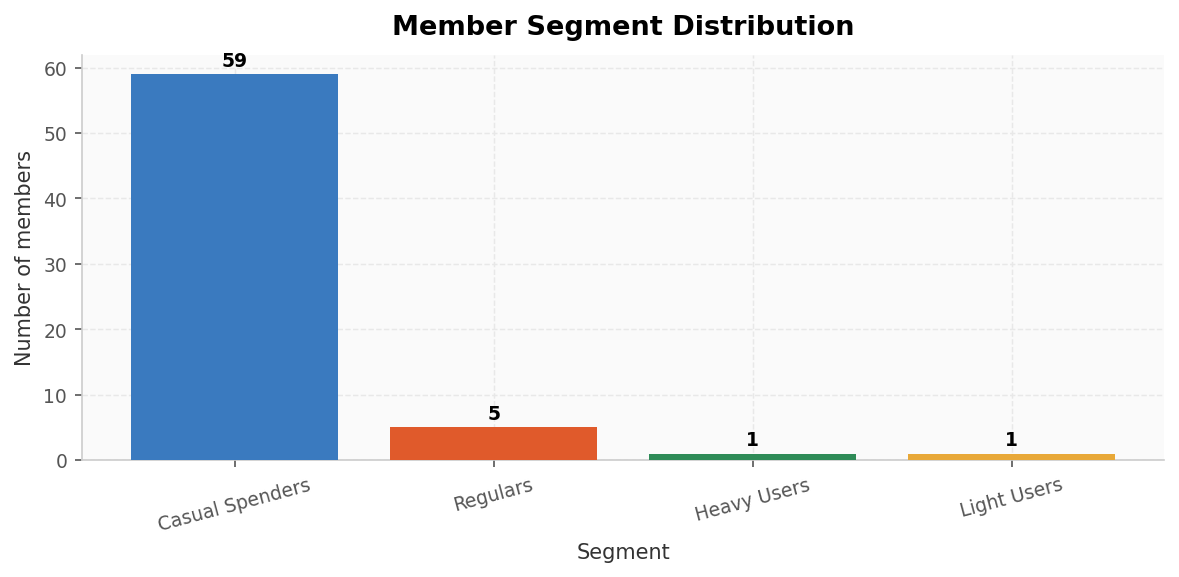
\includegraphics[width=0.65\textwidth]{segment_distribution.png}
  \caption{Distribution of the 66 members across the four
           segments.\label{fig:segment_dist}}
\end{figure}

\begin{table}[H]
  \centering
  \caption{Member segment distribution.\label{tab:segments}}
  \begin{tabular}{lrp{7cm}}
    \toprule
    \textbf{Segment} & \textbf{Members} & \textbf{Profile} \\
    \midrule
    Heavy Users     & -- & High spend, long sessions, high food orders \\
    Casual Spenders & -- & Shorter sessions, relatively high food orders \\
    Regulars        & -- & Balanced across all three features \\
    Light Users     & -- & Low spend and short sessions \\
    \bottomrule
    \multicolumn{3}{r}{\small\textit{Fill in member counts after running the pipeline.}} \\
  \end{tabular}
\end{table}

\section{Anomaly Detection}

\subsection{Motivation}

A dashboard shows what happened. It does not say whether what happened was normal.
A sharp drop in revenue on a Tuesday could mean a power outage, a recording error, or
simply a quiet day. Without a reference point, it is hard to tell.

The anomaly detection module provides that reference automatically. For each day in
the historical record, it calculates how unusual the revenue, session volume, and
member activity were relative to all other days of the same weekday. Days that fall
far outside the expected range are flagged, classified by severity, and exported for
review in Power~BI.

\subsection{Method --- Day-of-Week Z-Score}

The Z-score is a standard statistical measure of how many standard deviations a value
sits away from the mean. For each day, the calculation is:

\[
  z = \frac{\text{actual} - \mu_{\text{weekday}}}{\sigma_{\text{weekday}}}
\]

where $\mu_{\text{weekday}}$ and $\sigma_{\text{weekday}}$ are computed from all
historical days of the same weekday. A day is flagged if $|z| \geq 2.0$, capturing
roughly the most unusual 5\% of days per weekday group. At least four historical
data points per weekday are required before any flag is raised.

Two severity levels are defined:

\begin{itemize}
  \item \textbf{Mild} ($2\sigma$ to $3\sigma$) --- the day was unusual but not
        extreme. Could be natural variation or a minor event. Worth noting but not
        necessarily worth investigating.
  \item \textbf{Severe} (above $3\sigma$) --- statistically very unlikely by chance
        (less than 0.3\% of days). Something specific probably occurred: a power
        cut, a gaming tournament, a public holiday, or a recording error by a cashier.
\end{itemize}

\subsection{Why Day-of-Week Grouping Matters}

A gaming center has a clear weekly rhythm: Saturdays draw significantly more customers
than Tuesdays. Comparing a Saturday's revenue against the overall daily average would
flag almost every Saturday as anomalous --- which tells the owner nothing useful.

Grouping within weekdays means the baseline for each comparison reflects what is normal
\textit{for that specific day of the week}. An unusual Saturday is one that stands out
against all the other Saturdays in the historical record. This makes the flagging
practical: the owner can trust that a flagged day is genuinely out of the ordinary,
not just a consequence of the weekend effect.

\subsection{No Train/Test Split}

Unlike the forecasting models, anomaly detection does not use a train/test split. The
question being asked is not \textit{how accurate will the model be in the future?} but
\textit{which past days were statistically unusual?} All available data is used to
compute the baseline, because more data means a more accurate mean and standard
deviation. Nothing is held back, since there is nothing to predict.

\subsection{Three Series Monitored Independently}

The module runs the same Z-score logic on three series, each independently:

\begin{itemize}[noitemsep]
  \item \textbf{Revenue (TND)} --- daily sum of income transactions.
  \item \textbf{Session volume} --- daily count of all transactions.
  \item \textbf{Member activity} --- daily count of member-type transactions.
\end{itemize}

Each series uses its own per-weekday mean and standard deviation. An anomaly in
revenue has no effect on the session volume Z-score.

\begin{figure}[H]
  \centering
  % *TODO* Add a timeline chart of daily revenue: x-axis = date (7 months), y-axis = revenue TND. Plot as a line chart. Overlay anomaly days as coloured markers: red dots for severe (|z| > 3), orange dots for mild (2 < |z| <= 3). Generate with matplotlib using fact_transaction data + anomalies.csv.
  
\includegraphics[width=0.90\textwidth]{anomaly_timeline.png}
  \caption{Revenue anomalies detected over the seven-month period. Red markers are
           severe ($|z|>3$); orange markers are mild ($2<|z|\leq 3$).\label{fig:anomalies}}
\end{figure}

\subsection{Output}

All flagged days across all three series are written to \texttt{anomalies.csv}, sorted
from the most extreme to the least extreme Z-score. Each row records the date, the
series, the weekday, the actual value, the weekday mean, the weekday standard deviation,
the Z-score, the direction (high or low), and the severity.

The file is loaded into Power~BI as an additional table. A dedicated dashboard page
can filter by series and severity to give the owner a focused list of dates that
deserve a closer look.

\section{Output Files}

All analytics outputs are written to \texttt{output/forecasts/} at the end of the
pipeline run.

\begin{table}[H]
  \centering
  \caption{Analytics output files.\label{tab:output_forecasts}}
  \begin{tabular}{ll}
    \toprule
    \textbf{File} & \textbf{Contents} \\
    \midrule
    \texttt{forecast\_revenue.csv}       & Weekly and monthly revenue projections (TND) \\
    \texttt{forecast\_members.csv}       & Weekly and monthly member activity projections \\
    \texttt{peak\_hours\_by\_hour.csv}   & Avg transactions per hour of day (0--23) \\
    \texttt{peak\_hours\_by\_day.csv}    & Avg transactions per day of week \\
    \texttt{session\_volume.csv}         & Weekly and monthly activity volume projections \\
    \texttt{stock\_replenishment.csv}    & Per-item restocking recommendation \\
    \texttt{member\_segments.csv}        & Members with cluster ID and segment label \\
    \texttt{anomalies.csv}               & Flagged anomaly days across all three series \\
    \bottomrule
  \end{tabular}
\end{table}

\section{Sprint 4 Review}

\subsection{Deliverables}

\begin{itemize}
  \item \textbf{\texttt{gamefydb/forecaster.py}} --- five forecasting functions plus
        the evaluation helpers (\texttt{\_evaluate\_prophet},
        \texttt{\_evaluate\_sarima}, \texttt{\_print\_comparison}), each independently
        callable and returning a clean pandas DataFrame.
  \item \textbf{\texttt{gamefydb/segmenter.py}} --- the \texttt{segment\_members()}
        function implementing K-means clustering with automatic label assignment,
        silhouette score reporting, and StandardScaler normalisation.
  \item \textbf{\texttt{gamefydb/anomaly\_detector.py}} --- the
        \texttt{detect\_anomalies()} function implementing day-of-week Z-score
        detection across three series, with mild/severe severity classification.
  \item \textbf{Eight output CSV files} in \texttt{output/forecasts/}, all loadable
        directly into Power~BI as additional tables alongside the star schema.
  \item \textbf{Updated \texttt{run.py}} --- a single command produces the full star
        schema, all forecast outputs, the Prophet vs.\ SARIMA comparison, member
        segmentation, and anomaly detection in one pass.
  \item \textbf{\texttt{docs/ml\_choices\_explained.md}} --- an 11-section reference
        document explaining every algorithm choice, parameter decision, and evaluation
        methodology used in this sprint.
\end{itemize}

\subsection{Validation}

Each module was tested with automated tests before pipeline integration:

\begin{itemize}[noitemsep]
  \item \textbf{Forecaster}: 13 tests covering evaluation helpers, edge cases
        (too-short series, date mismatches), and metric signs. All passing.
  \item \textbf{Segmenter}: 12 tests covering label assignment, normalisation, and
        the all-zero member exclusion. All passing.
  \item \textbf{Anomaly detector}: 7 tests covering spike detection (severe), dip
        detection (mild), series isolation, small-group skipping, output columns, and
        sort order. All passing.
  \item \textbf{End-to-end}: the pipeline was run on the real dataset. All eight
        output files were loaded into Power~BI and verified. Flagged anomaly dates
        were cross-checked against the raw revenue chart to confirm they correspond
        to visually unusual days.
\end{itemize}

\section{Conclusion}

Sprint~4 added three analytical capabilities that move the system from description to
intelligence. Forecasting gives the owner a concrete planning window for the coming
weeks and months. The model comparison provides a reproducible, objective justification
for the algorithm choice. Member segmentation turns the loyalty dimension into four
actionable customer groups. Anomaly detection surfaces historical outliers and gives
the owner a systematic way to investigate unusual days rather than relying on chance
to notice them.

Together, these capabilities answer three questions the system could not answer before:
\textit{what is likely to happen next?}, \textit{who are the most valuable members?},
and \textit{which past days were out of the ordinary?}

% ============================================================
%  GENERAL CONCLUSION
% ============================================================
\chapter*{General Conclusion}
\addcontentsline{toc}{chapter}{General Conclusion}

This project set out to answer a practical question: how can the raw, artefact-laden
Excel exports of a gaming center be turned into a clean, reliable dataset that supports
real decision-making? The answer, delivered through four iterative sprints, is the
GamefyDB system.

Sprint~0 laid the foundations: a requirements specification, a Scrum framework, a
product backlog, and a dimensional model based on the Kimball approach. The decision
to use a star schema proved correct --- the resulting six-table structure is simple
enough for Power~BI to navigate without complex joins, yet complete enough to cover
all the KPIs the Product Owner needed.

Sprint~1 tackled the hardest part of the project: the source data itself. The four
\texttt{.xls} files were more problematic than initially anticipated. Page-break
artefacts repeated every 40 rows. An encoding issue in the members file required
switching from pandas to \texttt{xlrd} for direct cell-level reading. Amounts used a
narrow no-break space as a thousands separator that standard parsers did not recognise.
Merged cells shifted the actual data positions away from the apparent column headers.
Every one of these issues is documented and handled in the codebase. A future export
from the same management software can be processed without any code changes.

Sprint~2 produced the star schema. The design was refined during implementation when it
became clear that all stock records were outgoing sales with no restock entries, making
a dedicated stock fact table unnecessary. The final six-table schema --- four dimensions
and two facts --- is clean, correctly keyed, and exports with a single command.

Sprint~3 delivered the Power~BI report: four dashboard pages covering revenue
performance, terminal and cashier rankings, live operations, and shift-level reporting.
All measures were validated against the source data. The template file
(\texttt{SalesDashboard.pbit}) means the entire report can be refreshed with a new
pipeline run in minutes.

Sprint~4 extended the system into predictive and analytical territory through three
complementary machine-learning modules. \textbf{Forecasting} uses Prophet to produce
revenue, member activity, and session volume projections for horizons of four weeks and
three months, with confidence intervals that give the owner a planning range rather than
a single number. A rigorous \textbf{Prophet vs.\ SARIMA comparison} on an 80/20
chronological train/test split provides a reproducible, objective justification for the
model choice and demonstrates that with the current dataset size SARIMA is competitive,
a finding that will naturally change as more historical data accumulates. \textbf{K-means
member segmentation} groups the 66 loyalty members into Heavy Users, Casual Spenders,
Regulars, and Light Users based on their actual spending, visit duration, and food order
patterns --- enabling targeted promotions backed by data rather than intuition.
Finally, \textbf{anomaly detection} uses a day-of-week Z-score to flag historical
days where revenue, session volume, or member activity was unusually high or low for
that day of the week, giving the owner a systematic way to investigate operational
irregularities instead of noticing them by chance.

Several directions remain open for future development. The current pipeline reads
static Excel exports; connecting it directly to the management software's database
would enable automatic daily refreshes with no manual steps. The Prophet models would
benefit from a longer history --- the current seven months of data prevents reliable
yearly seasonality detection, and forecast accuracy is expected to improve beyond the
one-year mark. A lightweight web interface could expose the dashboards and analytics
to staff without requiring Power~BI Desktop. The member segmentation could be extended
with visit recency once per-visit timestamps become available, enabling a full RFM
(Recency, Frequency, Monetary) analysis as a fourth dimension.

Overall, GamefyDB demonstrates that a small business running on spreadsheets can gain
genuine analytical capability through a well-designed ETL pipeline and open-source
tooling. The center now has a repeatable, automated process that transforms its
operational data into a resource for real decision-making --- and a solid foundation
that can grow alongside the business.
